% =============== roughly chpt 4 ===============

\subsection{Shared synthetic data set across model types}
Fitting to the same synthetic data set, such that we may compare performance across model types for the same data set. 
This data was generated by a hand-engineered ...

\begin{figure}
    \centering
	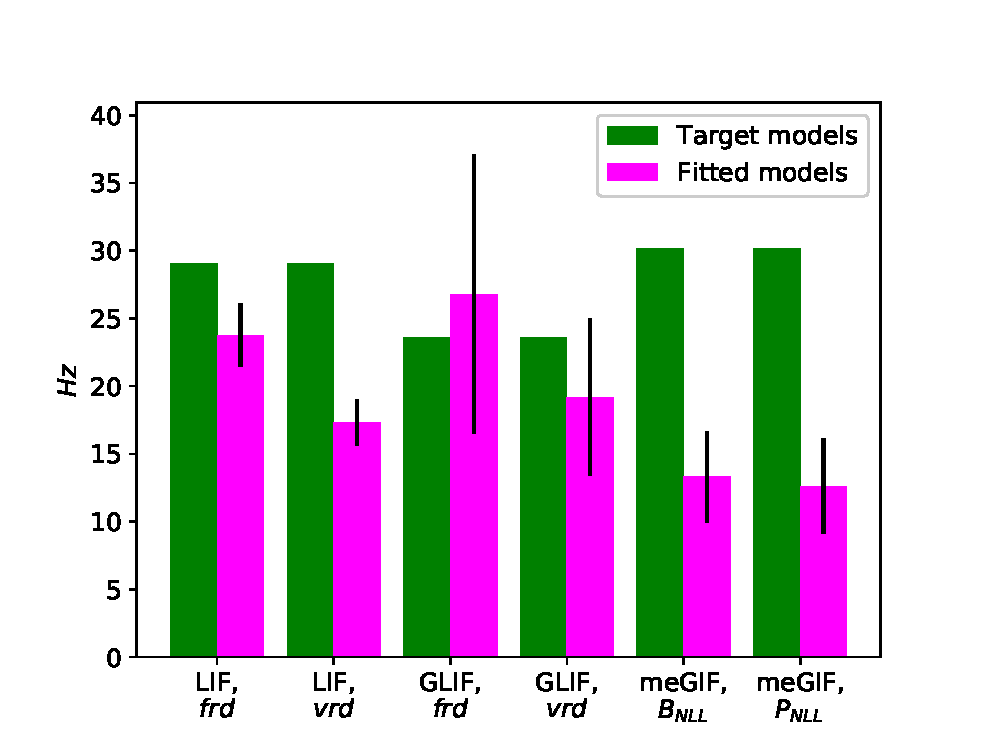
\includegraphics[width=0.49\columnwidth]{figures/export_rates_only_GT_all.eps}
\end{figure}

% \begin{figure}
% 	\includegraphics{figures/}
% \end{figure}


% \subsection{Leaky integrate-and-fire (LIF)}

% Gradient-based methods prone to finding sub-optimal solutions, i.e. local minimas. This is an issue particularly for high-dimensional feature spaces. Thus, I am led to believe this will be an issue when trying to infer the model parameters of complex neural networks using spike trains.

% %--------------------
% LIF work log:
% More nuanced
% Very noisy gradients for unstable/chaotic generative model perturbation?
% Dynamic R\_I in conjunction with frd might result in better convergence, due to constraining search space.
% By using dynamic R\_I (linear constraint), this makes behaviour more stable, and so may allow for more calibration/optimisation of the other parameters.

% % vRD suddenly seems viable for more stable network behaviour. When model behaviour was more chaotic, frd was better. This makes sense, as gradient will not be well-defined for vRD when model is chaotic. Not necessarily for frd either, but this is more robust to noise.

% Some artefacts LIF (more linear, easier to have whole-network spiking with too little inhibition / simpler neuron dynamics)

% Initial conditions large effect on convergence

% vRD performance OK with tau=100.0
% frd better
% In conjunction: still sometimes silent neurons. Potentially due to local minima of vRD for silent neurons, and obscured parameter-landscape due to noise and the nature of the vRD-metric. Not necessarily orthogonal to frd either, and as such may interfere with its gradient

% Will have to look at vRD vs frd vs frd+vRD vs adaptive(frd+vRD) quantitatively for setups.

% There seem to be many regions for which there is no “information gain” when moving along gradients, such as for silent neurons. Some parameters might not have their effect obscured or less pronounced due to the change of other parameters in parallel, too. This is the reason other authors have performed sequential parameter optimisation.

% When constructing generative target models, we aimed for hand-engineering models entraining higher-order ensemble dynamics that were stable across different random seeds of model perturbation, such that we could test how well model inference would capture these statistics. To this end, we designed three populations of neurons, where each population had different neuron parameters, normally distributed around set means, with a standard deviation of 25 % around the population values for each neuron. 
% In order to not generate spurious data, such as if the generative model is driven primarily by its input perturbation, or where it behaves otherwise chaotically, we tested that the hand-engineered models’ higher order statistics indeed occurred across different random seeds.

% (To verify that the model would indeed be sensible for synthetic generation, we tested the stability of neuron rates across different random seeds. When a deviation lower than X was attained, we accepted the ensemble model as a generative model suitable for data generation in order to test our framework.)
% Note that this deviation test is only to determine that the model doesn’t behave chaotically, and does not fire spuriously, in which case optimisation would be like fitting to noise, which should not converge.


% =============== roughly chpt 2 ===============
% The good old Bayes' rule:
% \begin{math}
%     P(\theta|X_o) = \frac{P(x_o|\theta)P(x_o)}{P(\theta)}
% \end{math}

% \section{(Evolutionary algorithms)}
% \section{Gradient free optimisation with evolutionary algorithms}

% I recall back to conferences talking about inferring complex, deep networks, which is a field where evolutionary algorithms (EAs) still are competitive and fruitful.
% In short, when EAs are fruitful, this often means the search space is so vast that gradient-based approaches will not converge.
% Even so, the computational cost is comparable, or even worse, than for ABC.

% NGO

% let's forget about casting the spike trains into a euclidean space, and propagating gradients. let's relax this to defined operations where there is a cost assigned to each operation, such that there is a minimal distance between two spike trains. this should let us define operations for moving single spikes, and shifting spikes. however, in my case there is uncertainty involved, so we should define operations for matching motifs instead. this makes it unclear for polynomial-time DP for calculating the distance. i can do pattern identification according to pre-defined rules, which will be exponential over a constant bound such that for longer time-intervals, a greedy comparison should be polynomial.
% if we assume that parts cannot cross in graph-matching, however, it becomes polynomial for the full distance-calculation (for larger intervals)

% sin (f(s)) + cos (g(s)) ?
% where f(s) = D\^spike[q, k]
% and g(s) = D\^interval[q, k]
% assume same labels?
% --> However, does not converge well.

% nevergrad + brian2
% for efficiency purposes..?
% Evolutionary algorithms may be used to traverse high-dimensional parameter-spaces in search for optimal solutions to complex problems such as fitting complex network models.
% This is made possible by by using objective functions to evaluate solution candidates, essentially provided as heuristics guiding the search. Note that finding the global optimum cannot be guaranteed when using evolutionary algorithms.
% In our case, due to the nature of the GLIF model, we may both constrain the parameter search space to meaningful parameter intervals, and employ search strategies that are more suited for the system.

% Two such evolutionary algorithm strategies are differential evolution (DE), and covariance matrix adaptation (CMA). 

% By using differential evolution (DE), a strategy where a set of best performing candidates are combined and mutated, we may continuously improve parts of the candidate solution, whilst potentially naturally constraining the search as a result.
% % revise the above
% While DE may be used to cross over and generate candidate solutions more broadly, it may also be skewed towards local optima. Another approach that we selected that might be better suited for very high-dimensional problems, is covariance matrix adaptation (CMA) evolution \cite{Igel2007}. CMA will naturally utilise correlated parameters in the model system as is the case in the GLIF model, and incorporates this by updating a covariance matrix during search path traversal, which is in turn used to maximise the probability for finding successful candidate solutions.
% Effectively, CMA does principal components analysis over its evolution path, which allows for variance and step size adjustment.
% CMA evolutionary strategies have been shown to perform well for difficult functions with larger budgets \cite{Hansen2010}.
% % revise the above

% % PSO, NGO?
% Initial testing with particle-swarm optimisation (PSO), which can be said to search more widely before converging towards the best performing candidate in the fitness landscape.
% However, divergence or non-converging bad fits, likely due to the vast complexity of the parameter-space and the nature of PSO.
% Failure to converge to results of comparable loss to the other optimisers was also the case with neighbourhood and genetic operator (NGO) search.




% -----------------------
% \subsection{Relaxing the constraint of differentiability}

% mostly if EAs??
% non GBO, but still ABC.

% permutations

% ...

% high-cost, not necessarily better due to stochasticity. 

% unknown input.

% may be studied further, but would require a large amount of computational resources, and it is currently unclear whether such endeavours would be fruitful. % ..?

% ---------------------
% \textbf{Something you can learn about network, but also should be specific to a spiking net
% Want to find something only in SNN, but which is also identifiable
% Don’t need to find exact same sync act., not same identities of neurons which participate, just general properties, in spite of unknown input activity}

% Advantages of SNNs compared to rate based/mean field
% Quantity
% Model statistics exhibited regardless of configuration
% Different inputs and generative model output variability

% “Vector strength is the Fourier component of the spike sequence at the stimulus frequency normalized by the total number of spikes”

% “It has been proposed that membrane time con- stant, spiking threshold, and the number of inputs per period are key parameters that determine the performance of a coincidence detector (Kempter et al. 1998)”
% On temporal info coded by phase-locked spikes processed in higher-order centers in the brain

% Precise firing sequence
% “Inappropriate surrogate” - high-order gamma dist great number of chance patterns due to generating quasiperiodic spike trains. Poissonian more unrelated periodic spike trains
% “Nonprecise time patterns” - interested in spike patterns (not one less precise peak in 3d corr M)

% (Analysis and interpretation of interval and count variability in (single neuron) neural spike trains
% Coefficient of variation (CV), trial-by trial count variability with the Fano factor (FF), estimation bias, …
% Variability on tens to hundreds of ms
% CV = SD(X)/E(X))

% Can we detect statistics relating to state in data using more sophisticated rate measures when compared to straightforward mean binned rates per state? Could this be used further?

% System. Spike train assumed to be distributed according to some distribution. Can invert and calculate probability and minimise. Fluctuation can for instance be regarded as due to “irregularity in time from a constant rate or regularly from a fluctuating rate”.
% Metric measuring ISI variability rescaled locally in time can suggest which is more plausible.
% When looking at more complex system this is less trivial..? MIght be used on higher-level such as neuron classes?

% Need to go beyond renewal processes to capture different neuronal modes of behaviour, and spike train adaptation - serial correlations in ISIs is one such step
% Hidden Markov processes, drawn from distribution relative to state
% “Memory” in nesting the probability such that it depends on N preceding ISIs

% Grün and Rotter, methods
% Characteristics that are stable in spite of different inputs

% Null hypothesis: Independence (spike trains)
% stochastic spike train models, posits probabilistic model for timing of spikes, based on the spike history. Simplest such; Poisson process.
% p(spike\_[t, t+dt]) ~~ Rdt, where R is the rate (for sufficiently small dt)
% Point processes for several spike trains (networks and not just neurons); papers (ignored here)
% ---------------------